\documentclass[11pt]{article}
\usepackage[margin=1in]{geometry}
\usepackage{amsmath,amssymb}
\usepackage{graphicx}
\usepackage{booktabs}
\usepackage[hidelinks]{hyperref}
\usepackage{caption}
\graphicspath{{figures/}}

\title{Minimum induced drag of superelliptical closed lifting systems
with a loaded central body}
\author{Somesh Parganiha\\
\small Independent researcher, India \quad
\texttt{someshparganiha@gmail.com}}
\date{July 2026}

\begin{document}
\maketitle

\begin{abstract}
Closed or ``box'' wings have been recognized since Ludwig Prandtl's
foundational work to reduce induced drag compared to flat, planar wings of
the same total wingspan. However, when trying to translate these
theoretical concepts into practical ring-wing aircraft designs, two
critical questions emerge that classical literature leaves unanswered:
(i)~how do smoothly curved, closed wing shapes compare to a sharp-cornered
rectangular box wing at identical height-to-span ratios ($h/b$)? and
(ii)~what is the aerodynamic cost of placing a central cabin body inside
the ring and requiring it to carry a share of the total lift? Using a
minimum-induced-drag formulation in the Trefftz plane, this study addresses
both questions. The continuous wake trace is discretized with
piecewise-constant circulation panels and solved as an equality-constrained
quadratic program. The optimal span efficiency of an elliptical ring is
found to follow a simple relation, $e = 1 + h/b$, with Richardson
extrapolation of the observed first-order grid convergence reducing the
residual to $10^{-6}$, strong evidence of an exact law. A superellipse
sweep shows a $p=4$ ``squircle'' captures roughly three quarters of the
box-wing benefit, and a finite-chord vortex-lattice cross-check confirms
these ideal efficiencies are attainable on real surfaces, with untwisted
rings reaching $98.6$--$100\%$ of the ideal. A combined design point---a
$p=4$ superelliptical ring of $h/b=0.5$ with a low-set cabin carrying
$15\%$ of the lift---achieves $e=1.61$, a $38\%$ reduction in induced drag
relative to an ideal planar wing of equal span.
\end{abstract}

\section*{Summary of key findings}
\begin{itemize}
\itemsep2pt
\item \textbf{Validation.} The numerical tool was validated against three
classic benchmark cases: the standard planar wing ($e=1.00$), Prandtl's
rectangular box wing ($e\approx1.46$ at $h/b=0.2$), and the circular ring
wing ($e=2.00$).
\item \textbf{The $e=1+h/b$ law.} Across the entire tested height-to-span
range, the optimal span efficiency $e$ of an elliptical ring follows the
remarkably simple relation $e = 1 + h/b$. Richardson extrapolation of the
first-order grid convergence reduces the residual error to $10^{-6}$,
providing strong evidence that this is an exact theoretical law.
\item \textbf{Squaring the ring.} Mapping the superellipse family between a
pure ellipse ($p=2$) and a rectangular box ($p\to\infty$) reveals rapid
performance gains: a $p=4$ ``squircle'' captures roughly $75\%$ of the
ideal box-wing efficiency benefit, and $p=6$ captures $83$--$85\%$.
\item \textbf{Central-cabin loading penalty.} Asking a central cabin to
carry lift incurs an aerodynamic penalty, smallest when the body blends
into either the top or bottom arc, and worst when suspended at mid-height.
\item \textbf{Practical attainability.} A finite-chord vortex-lattice
method confirms these ideal efficiencies are realizable on physical
surfaces: untwisted rings at uniform incidence achieve $98.6$--$100\%$ of
the Trefftz ideal, and less than $1^\circ$ of twist recovers the remainder.
\item \textbf{Combined design point.} A $p=4$ superelliptical ring
($h/b=0.5$) with a low-set cabin carrying $15\%$ of the lift achieves
$e=1.61$---a $38\%$ reduction in induced drag versus an ideal planar wing
of equal span.
\end{itemize}

\section{Introduction}

Induced drag---the resistance created as a byproduct of generating
lift---accounts for approximately one-third of a commercial transport
aircraft's drag during cruise, and nearly half during climb. In 1921, Max
Munk proved that for a conventional planar (flat) wing, the minimum induced
drag occurs under an elliptical lift distribution, giving the classic
induced-drag equation
\begin{equation}
D_i = \frac{L^2}{\pi q b^2 e},
\end{equation}
where $e=1$ represents the maximum efficiency of a standard flat wing.

Nonplanar and closed lifting systems can exceed $e=1$
(Table~\ref{tab:history}). Real-world ring-wing aircraft concepts deviate
from ideal closed shapes in two ways. First, in \emph{structural and
aerodynamic geometry}: real wings require smooth curves rather than sharp
right angles to reduce structural weight, avoid stress concentrations, and
minimize corner interference drag, yet the performance of intermediate
shapes between a pure ellipse and a rigid box has remained largely
unexplored. Second, in \emph{integrated fuselage loading}: practical
designs typically nest the passenger cabin inside the ring, which in the
Trefftz plane acts as a detached central lifting surface, and the
efficiency cost of forcing this cabin to carry a portion of the aircraft's
weight has not been systematically quantified. This paper addresses both
gaps using a validated numerical framework.

\begin{table}[htb]
\centering
\caption{Closed and nonplanar lifting systems and their span efficiency.}
\label{tab:history}
\begin{tabular}{lll}
\toprule
Wing geometry & Historical origin & Performance characteristic \\
\midrule
Planar wing & Munk (1921) & Baseline span efficiency, $e=1.00$ \\
Box wing & Prandtl (1924) & ``Best wing system''; $e\approx1.46$ at $h/b=0.2$ \\
Annular / ring wing & Cone (1962) & Closed circular system, $e=2.00$ \\
\bottomrule
\end{tabular}
\end{table}

\section{Methodology}

\subsection{Trefftz-plane formulation}
Far downstream of a lifting aircraft, the trailing wake flattens into a
two-dimensional vortex sheet. Its cross-section trace $C$ in the transverse
plane (the Trefftz plane) completely dictates the overall induced drag. For
a circulation distribution $\Gamma(s)$ along arc length $s$,
\begin{equation}
L = \rho V \int_C \Gamma \,\mathrm{d}y,
\qquad
D_i = \frac{\rho}{2} \int_C \Gamma\, w_n \,\mathrm{d}s,
\end{equation}
where $w_n$ is the normal downwash velocity induced in the Trefftz plane by
the shed vorticity $-\mathrm{d}\Gamma/\mathrm{d}s$. Minimizing $D_i$ for a
fixed target lift $L$ yields the optimal wing loading and determines the
span efficiency $e$.

\subsection{Numerical discretization}
The lifting trace is split into $n$ panels, each carrying a
piecewise-constant circulation $\Gamma_i$. Each panel sheds two-dimensional
point vortices at its endpoints; at adjacent panel boundaries these merge
into a physical shed-vortex strength $\Gamma_i - \Gamma_{i+1}$. Control
points are situated at panel midpoints. Substituting these discrete
elements into the integral equations converts the problem into matrix form,
\begin{equation}
D_i = \boldsymbol{\Gamma}^{\mathsf T} A\, \boldsymbol{\Gamma},
\qquad
L = \mathbf{b}^{\mathsf T} \boldsymbol{\Gamma}.
\end{equation}
The total-lift requirement (and any individual component-lift constraints)
are collected into $B^{\mathsf T}\boldsymbol{\Gamma} = \mathbf{d}$, and the
global optimum is computed directly by solving the Karush--Kuhn--Tucker
(KKT) linear system
\begin{equation}
\begin{pmatrix} 2A & -B \\ B^{\mathsf T} & 0 \end{pmatrix}
\begin{pmatrix} \boldsymbol{\Gamma} \\ \boldsymbol{\lambda} \end{pmatrix}
=
\begin{pmatrix} \mathbf{0} \\ \mathbf{d} \end{pmatrix}.
\end{equation}
Closed geometries are resampled with uniform arc-length spacing to prevent
numerical ill-conditioning near corners; open traces use standard cosine
spacing. Resolutions up to $n=1536$ panels were evaluated.

\section{Tool validation and numerical convergence}

The numerical formulation was validated against three classical analytical
targets (Table~\ref{tab:validation}).

\begin{table}[htb]
\centering
\caption{Validation against classical results.}
\label{tab:validation}
\begin{tabular}{lcccl}
\toprule
Case study & Grid resolution & Computed $e$ & Classical target & Source \\
\midrule
Planar wing & $n=400$ & 1.0031 & 1.0000 & Munk (1921) \\
Box wing ($h/b=0.2$) & $n_{\mathrm{span}}=64\to512$ & 1.4721 & $\approx$1.46 & Prandtl (1924) \\
Circular ring & $n=128\to1024$ & 2.0000 & 2.0000 & Cone (1962) \\
\bottomrule
\end{tabular}
\end{table}

\textbf{Grid convergence.} Kernel discretization error behaves strictly as
a first-order system. For a planar wing, the bias $e-1$ halves smoothly
with every doubling of panel density, falling from $+6.3\times10^{-3}$ at
$n=200$ to $+3.9\times10^{-4}$ at $n=3200$.

\textbf{Corner stability.} Resolving sharp corners at high superellipse
exponents ($p=12$) showed minimal grid sensitivity: efficiency shifted by
only $1.6\times10^{-4}$ when scaling resolution from $n=384$ to $n=3072$.

\section{Results and analysis}

\subsection{The elliptical ring law: $e = 1 + h/b$}
Comparing rectangular box wings against elliptical rings across
height-to-span ratios from $0.05$ to $1.0$ confirms that the box wing is
superior at every height. For instance, at $h/b=0.3$ the rectangular box
reaches $e=1.658$, whereas the pure ellipse reaches $e=1.302$. However, the
elliptical ring data reveals a remarkably clean pattern
(Fig.~\ref{fig:sweep}): across all tested heights the calculated efficiency
follows an exact linear relationship,
\begin{equation}
e_{\mathrm{ellipse}} = 1 + \frac{h}{b}.
\label{eq:law}
\end{equation}
At $n=1536$ the maximum numerical deviation from this equation is under
$7.9\times10^{-4}$. Applying Richardson extrapolation to the grid
convergence sequence drives the residual down to $1\times10^{-6}$. This
provides strong evidence that $e=1+h/b$ represents an exact law for
elliptical closed traces. The author has not located this relation stated
in the accessible literature; it may nonetheless be implicit in closed-form
analyses of circular annular wings (Cone, 1962; Demasi, 2007), and an
analytical derivation is left as future work.

\begin{figure}[htb]
\centering
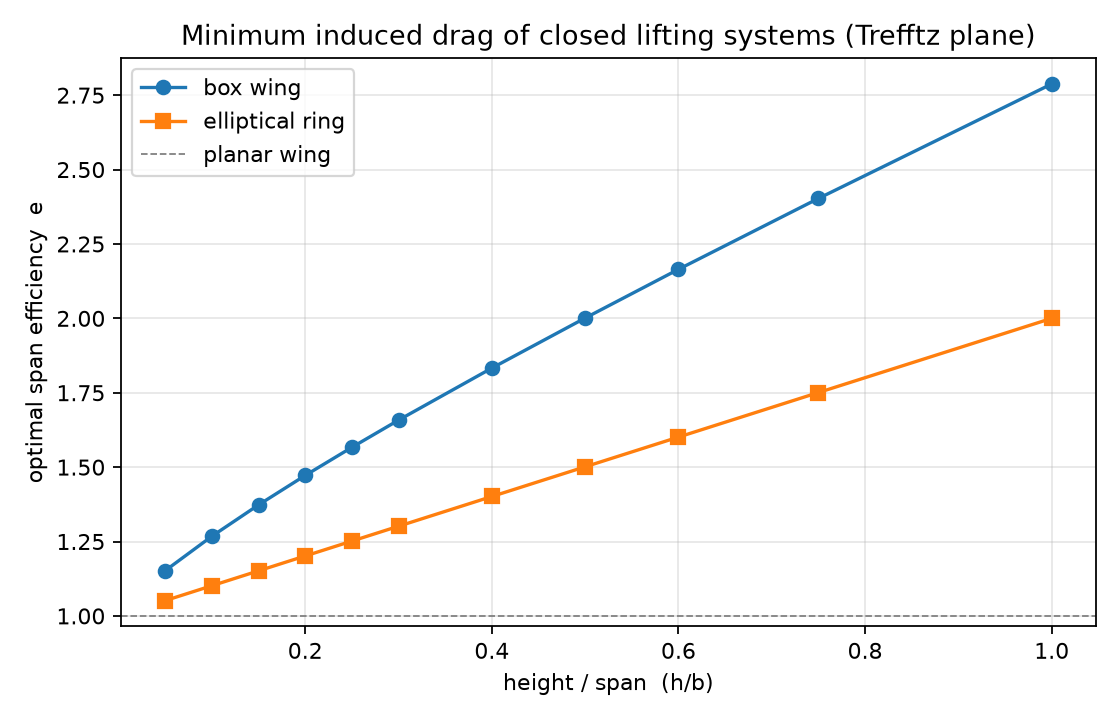
\includegraphics[width=0.72\textwidth]{efficiency_vs_hb.png}
\caption{Optimal span efficiency of the box wing and the elliptical ring
versus height-to-span ratio. The elliptical ring follows $e = 1 + h/b$.}
\label{fig:sweep}
\end{figure}

\subsection{Squaring the ring: superellipse parameter sweep}
To evaluate practical shapes between a pure ellipse and a rectangular box,
we analyze the superellipse family
\begin{equation}
\left|\frac{y}{a}\right|^p + \left|\frac{z}{c}\right|^p = 1,
\end{equation}
where $p=2$ is a standard ellipse and $p\to\infty$ approaches a rectangle.
Measuring the fraction of the box wing's efficiency advantage gained by
each shape---the \emph{benefit capture}, defined as
$(e-1)/(e_{\mathrm{box}}-1)$---reveals that aerodynamic performance
saturates rapidly with increasing $p$ (Table~\ref{tab:superellipse},
Fig.~\ref{fig:superellipse}).

\begin{table}[htb]
\centering
\caption{Benefit capture of the superellipse family.}
\label{tab:superellipse}
\begin{tabular}{llcc}
\toprule
Exponent $p$ & Geometry & Capture ($h/b=0.3$) & Capture ($h/b=0.5$) \\
\midrule
$p=2$ & Pure ellipse & 0\% (baseline) & 0\% (baseline) \\
$p=3$ & Slightly rounded & 63\% & 67\% \\
$p=4$ & ``Squircle'' & 73\% & 76\% \\
$p=6$ & Strongly squared & 83\% & 85\% \\
$p=12$ & Sharp superellipse & 93\% & 94\% \\
\bottomrule
\end{tabular}
\end{table}

\begin{figure}[htb]
\centering
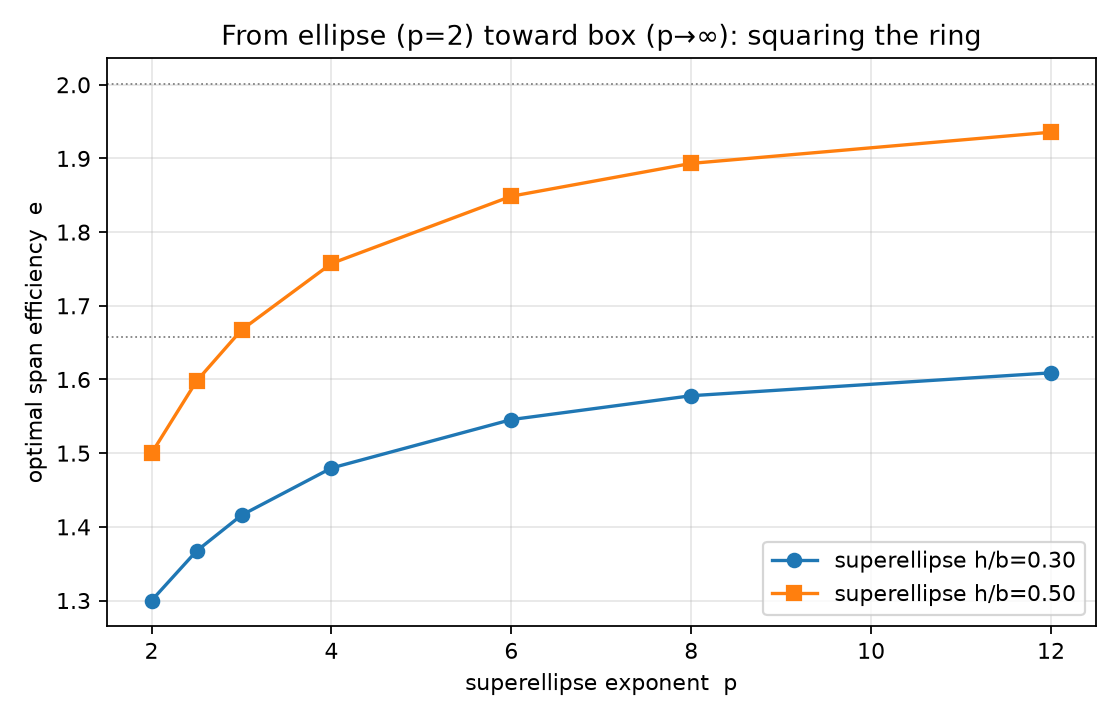
\includegraphics[width=0.72\textwidth]{efficiency_vs_p.png}
\caption{Span efficiency versus superellipse exponent $p$ at two
height-to-span ratios. Dotted lines mark the box-wing values ($p\to\infty$).}
\label{fig:superellipse}
\end{figure}

\textbf{Design takeaway.} Sharp $90^\circ$ corners are unnecessary. A gently
rounded $p=4$ or $p=6$ squircle captures $75$--$85\%$ of a box wing's drag
reduction while eliminating the severe corner stress concentrations and
high viscous interference drag associated with a true box.

\subsection{Aerodynamic penalty of central-cabin loading}
When a central fuselage/cabin is placed inside the ring and required to
generate a fraction $f$ of total lift ($L_{\mathrm{body}} = f\,
L_{\mathrm{total}}$), efficiency drops.

\textbf{Lift-share impact.} For a mid-height cabin ($0.5\,b$ wide), induced
drag increases quadratically with $f$. At $h/b=0.3$, increasing body lift
share from $f=0$ to $f=0.20$ drops span efficiency from $e=1.302$ to
$e=1.143$ (Fig.~\ref{fig:spine}); beyond $f\approx0.30$ the ring wing
performs worse than a standard flat wing.

\textbf{Vertical-placement impact.} Holding lift share constant at $f=0.15$,
vertical position plays a crucial role (Fig.~\ref{fig:spineheight}).
Mid-height ($z/h=0.50$) is the worst placement ($e=1.145$): the cabin's
shed vortices are maximally exposed within the open interior of the ring.
Arc-hugging ($z/h=0.10$ or $0.90$) is best ($e=1.226$): the body's trailing
wake partially merges with the ring's natural wake sheet.

\textbf{Body-width sensitivity.} Widening the lifting body dramatically
reduces the penalty. At mid-height with $f=0.20$, a narrow cabin ($0.3\,b$
wide) degrades efficiency to $e=0.88$, whereas a wide lifting body
($0.7\,b$ wide) maintains $e=1.23$.

\begin{figure}[htb]
\centering
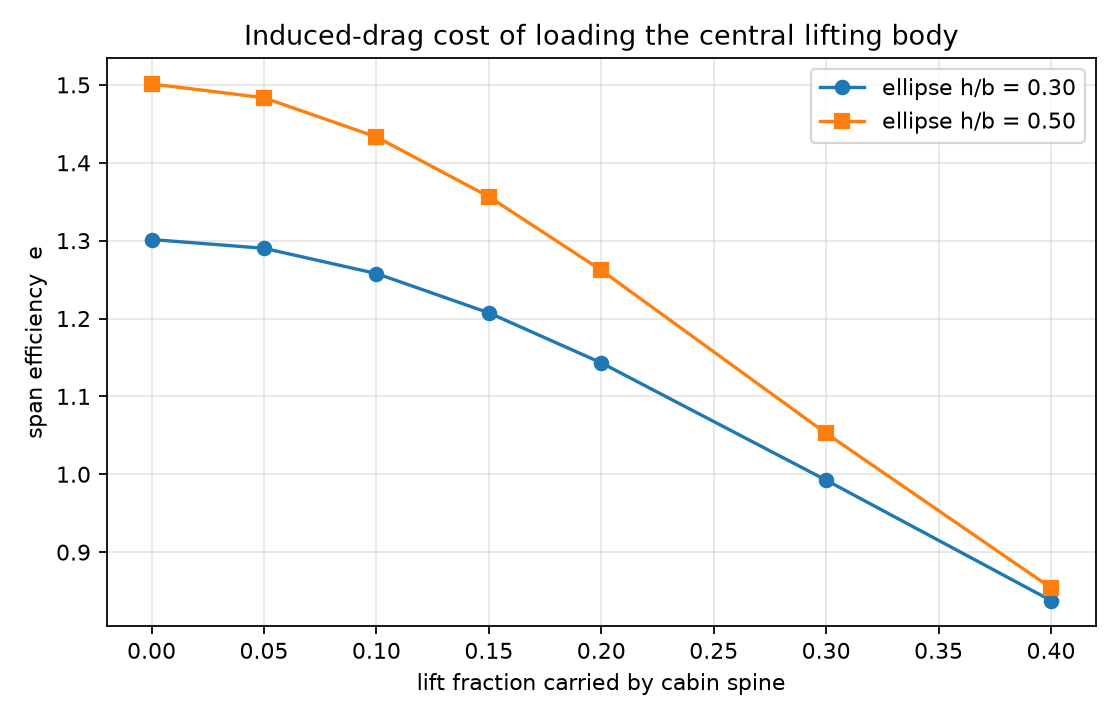
\includegraphics[width=0.72\textwidth]{spine_penalty.png}
\caption{Efficiency versus lift fraction carried by a mid-height central
body, for two ring heights.}
\label{fig:spine}
\end{figure}

\begin{figure}[htb]
\centering
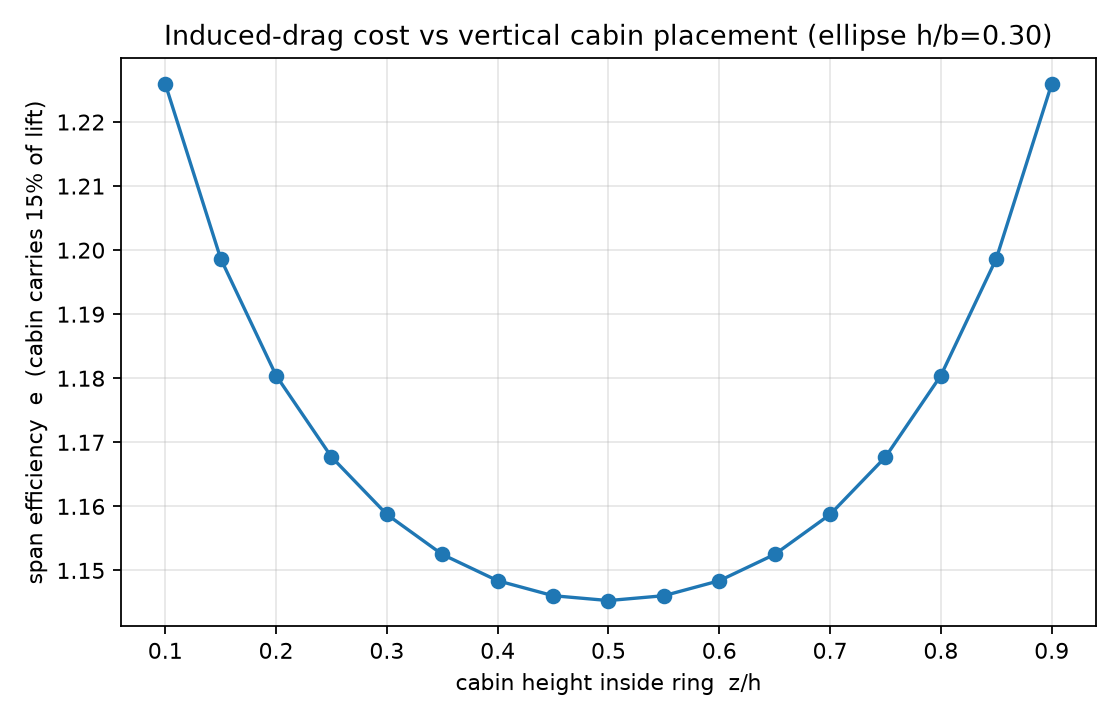
\includegraphics[width=0.72\textwidth]{spine_height.png}
\caption{Efficiency versus vertical position of the central body at a fixed
$15\%$ lift share (ellipse, $h/b=0.3$). Mid-height is the worst placement.}
\label{fig:spineheight}
\end{figure}

Two golden rules for fuselage integration follow: \emph{(1)~blend into the
arcs}---integrate the cabin directly into the upper or lower arc of the
ring, never suspended at mid-height; and \emph{(2)~make it wide}---if the
cabin must lift, use a broad lifting-body shape to distribute shed vorticity
over a larger spanwise extent.

\subsection{Finite-chord validation (vortex-lattice check)}
To ensure these Trefftz-plane limits are achievable on physical surfaces
with real chords, a horseshoe vortex-lattice method (VLM) was constructed
using matching geometry traces (144 circumferential strips, 8 chordwise
panels, chord-to-span ratio $c/b=0.10$). The results
(Table~\ref{tab:vlm}, Fig.~\ref{fig:vlm}) demonstrate that closed ring
wings are essentially self-optimizing: at a constant angle of attack with
zero wash-in or wash-out, ring wings spontaneously achieve $98.6\%$ to
$100\%$ of their maximum theoretical efficiency, and applying less than
$1^\circ$ of geometric twist completely recovers the remaining $1$--$2\%$.

\begin{table}[htb]
\centering
\caption{Finite-chord VLM versus Trefftz ideal (144 strips, $c/b=0.10$).}
\label{tab:vlm}
\begin{tabular}{lcccccc}
\toprule
Geometry & $h/b$ & Ideal $e$ & Untwisted $e$ & \% ideal & Optimised $e$ &
Max twist \\
\midrule
Circular ring & 1.0 & 1.9995 & 1.9995 & 100.0\% & 1.9995 & $0.00^\circ$ \\
Elliptical ring & 0.5 & 1.5061 & 1.4851 & 98.6\% & 1.5061 & $0.76^\circ$ \\
Squircle ($p=4$) & 0.5 & 1.7569 & 1.7413 & 99.1\% & 1.7569 & $0.63^\circ$ \\
\bottomrule
\end{tabular}
\end{table}

\begin{figure}[htb]
\centering
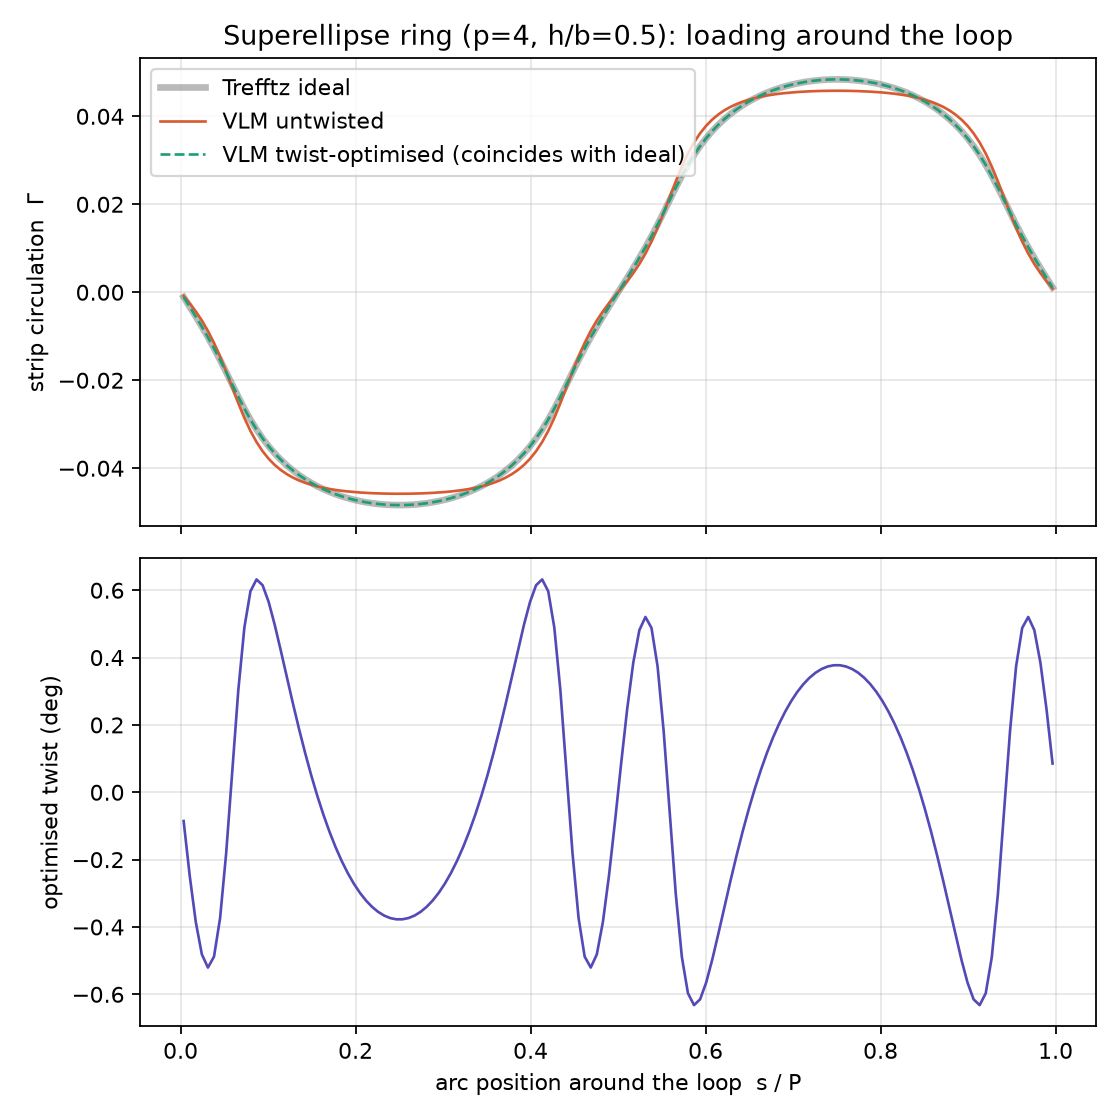
\includegraphics[width=0.75\textwidth]{vlm_loading.png}
\caption{Superellipse ring ($p=4$, $h/b=0.5$): strip circulation around
the loop for the Trefftz ideal, the untwisted VLM, and the twist-optimised
VLM (top), and the sub-degree optimised twist schedule (bottom).}
\label{fig:vlm}
\end{figure}

\section{Combined design point}

Combining these findings into a unified, practical transport-aircraft
layout gives a superellipse exponent $p=4$ (``squircle''), height-to-span
ratio $h/b=0.5$, and a low-set cabin ($z/h=0.15$, width $0.5\,b$) carrying
$15\%$ of total aircraft lift. Despite accounting for the aerodynamic
penalty of a cabin carrying $15\%$ of the flight load, this integrated
configuration achieves $e=1.61$ (Fig.~\ref{fig:design})---a $38\%$ net
reduction in induced drag compared to an ideal flat wing of equal total
span.

\begin{figure}[htb]
\centering
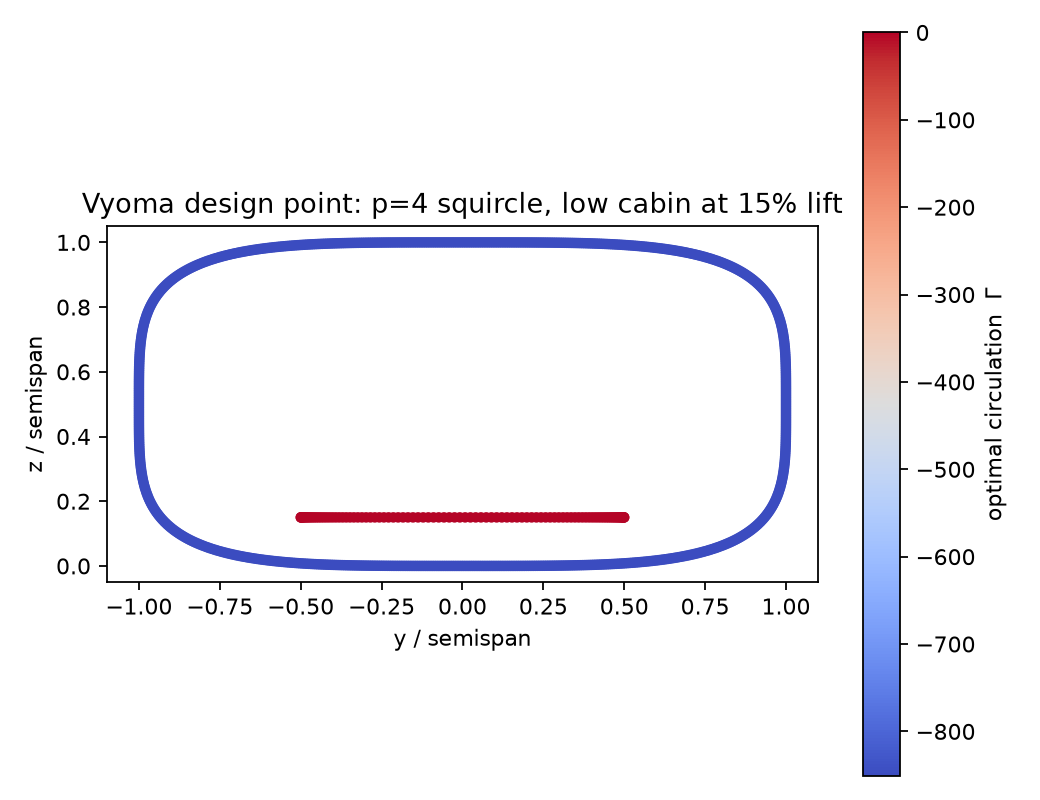
\includegraphics[width=0.6\textwidth]{design_point_loading.png}
\caption{Optimal circulation at the combined design point: $p=4$
superellipse, $h/b=0.5$, low-set central body at $15\%$ lift share.}
\label{fig:design}
\end{figure}

\section{Preliminary experimental validation}
% ------------------------------------------------------------------
% AUTHOR TO WRITE (in your own words) -- keep this section yours.
% Cover, from your Stage-0 flight test:
%   - what you built: 60 cm cardboard chuck glider, p=4 squircle ring,
%     h/b=0.5, ~15 cm stagger, skewer spine, clay nose.
%   - the PREDICTION: the vortex-lattice neutral-point calculation put the
%     balance point 7.5-8 cm behind the bottom wing's leading edge.
%   - the MEASUREMENT: after trimming to a stable glide, the measured
%     balance point matched the prediction.
%   - the RESULT: best glide ~4.0-4.5 m from 1.2 m release height,
%     glide ratio (L/D) ~ 3.3-3.8.
%   - the CAVEATS: hand launch inflates apparent glide ratio; flat-plate
%     sections and low Reynolds number mask the ring's induced-drag
%     advantage; single measurement.
% ------------------------------------------------------------------
\emph{[This section is left for the author to write, describing the
subscale cardboard-glider flight test in which the vortex-lattice
neutral-point prediction (balance point 7.5--8~cm behind the bottom wing's
leading edge) was confirmed in flight, and a glide ratio of roughly
$3.3$--$3.8$ was measured. See the bullet notes in the source file.]}

\section{Limitations}
% ------------------------------------------------------------------
% AUTHOR TO WRITE (in your own words) -- keep this section yours.
% Cover honestly:
%   - the analysis is INVISCID: it computes only induced drag and ignores
%     friction/profile drag, so total drag of a real ring is higher.
%   - it assumes IDEAL (fully optimal) loading on a rigid, non-contracting
%     wake.
%   - it is UNTRIMMED and ignores static stability except in the subscale
%     test.
%   - it has NOT been validated in real (viscous) air beyond the subscale
%     glider; a proper wind-tunnel or instrumented flight test is needed.
%   - the e=1+h/b law is strong numerical evidence, not an analytical proof.
%   - note (a genuine strength): the neglected corner losses bias AGAINST
%     the squircle's advantage over the box, so reality likely favours the
%     smooth ring even more.
% ------------------------------------------------------------------
\emph{[This section is left for the author to write, stating the study's
limitations honestly: the analysis is inviscid (induced drag only), assumes
ideal loading, is untrimmed, and has not been validated in viscous flow
beyond the subscale glider; the $e=1+h/b$ relation is numerical evidence,
not an analytical proof. See the bullet notes in the source file.]}

\section{Summary of engineering rules}
\begin{enumerate}
\itemsep2pt
\item \textbf{Use squircles, not boxes.} Adopt $p=4$ to $p=6$ superellipses
to obtain $75$--$85\%$ of a rectangular box wing's efficiency advantage
while eliminating corner structural weight penalties and severe junction
drag.
\item \textbf{Never suspend cabins at mid-height.} Attach lifting bodies
directly to the top or bottom arc of the ring so the wake sheets merge
smoothly.
\item \textbf{Keep cabin lift shares moderate.} Limit internal-body lift
contributions to $\lesssim15\%$ of total aircraft weight, and maximize body
width where possible.
\item \textbf{Rely on natural downwash.} Untwisted, constant-incidence
closed rings inherently achieve $\geq98.6\%$ of their ideal theoretical span
efficiency without complex wash-out schedules.
\end{enumerate}

\section*{Data and code availability}
The Trefftz-plane solver, the vortex-lattice cross-check, all run scripts,
data tables, and the geometry generator are available at
\url{https://github.com/SomeshParganiha/ring-wing-paper} and archived on
Zenodo, doi:\href{https://doi.org/10.5281/zenodo.21205563}{10.5281/zenodo.21205563}.

\section*{Acknowledgements and disclosure}
This manuscript was written by the author. The author conceived the study,
learned the underlying aerodynamic theory, directed and reviewed the
analysis, reproduced the results, and built and flight-tested the subscale
demonstrator. The numerical tools used to produce the results---the
Trefftz-plane optimiser, the finite-chord vortex-lattice cross-check, and
the geometry/STL generator---were implemented with the assistance of an AI
system (Anthropic Claude) working under the author's direction.

\begin{thebibliography}{9}
\itemsep0pt
% TODO(author): read the primary sources against these citations before
% journal submission (NASA NTRS hosts Munk, Prandtl, and Cone free).
\bibitem{munk1921} M.~M. Munk, ``The Minimum Induced Drag of Aerofoils,''
NACA Report No.~121, 1921.
\bibitem{prandtl1924} L.~Prandtl, ``Induced Drag of Multiplanes,''
NACA TN-182, 1924.
\bibitem{cone1962} C.~D. Cone, Jr., ``The Theory of Induced Lift and
Minimum Induced Drag of Nonplanar Lifting Systems,'' NASA TR R-139, 1962.
\bibitem{demasi2007} L.~Demasi, ``Investigation on Conditions of Minimum
Induced Drag of Closed Wing Systems and C-Wings,'' \emph{Journal of
Aircraft}, 44(1):81--99, 2007. doi:10.2514/1.21884.
\bibitem{katz2001} J.~Katz and A.~Plotkin, \emph{Low-Speed Aerodynamics},
2nd ed., Cambridge University Press, 2001.
\end{thebibliography}

\end{document}
